%% Original Template Author: Robin Turner, Adapted from the IEEE peer review template
%% by Luca Dalmasso
%% 

\documentclass[a4paper]{report}
\usepackage[utf8]{inputenc} % Allows Turkish characters.
\usepackage{booktabs} % Allows the use of \toprule, \midrule and \bottomrule in tables for horizontal lines
\usepackage{graphicx}
\usepackage{xcolor}


\begin{document}
\title{GPU programming \\ LeNet-1 Project Report}
\author{Dalmasso Luca\\
        Computer Engineering, Embedded Systems master degree\\
        Politecnico of Turin
        }

\date{01/07/2022}

% make the title area
\maketitle
\tableofcontents
\listoffigures
\listoftables

%\end{titlepage}

%\IEEEpeerreviewmaketitle
\begin{abstract}
This project consists in developing the LeNet-1 Convolutional Neural Network with the aim of speeding it up in a GPU through the CUDA programming language.\\
In this report is presented one possible implementation of the CNN on the GPU that starts from a very naïve version of the algorithm and shows what are the optimisations that were implemented in order to get better performances and better usage of the GPU resources.

\end{abstract}

\section{Introduction}
In the domain of Machine Learning, Convolutional Neural Networks (CNNs) are particular class of  Depp Learning algorithms specifically designed to process pixel data and so  widely used for image classification and object recognition.
The LeNet-1 is a CNN architecture introduced in 1998 by Yann LeCun and other researchers as an attempt to classify 2D images, in particular with the purpose of recognising handwritten digits in ZIP codes.

%%%CAP 2 BACKGROUND %%%%%
\section{Background}
A very general architecture of a CNN is the one showed in Figure 1 where it is possible to see that, from a general point of view, a CNN is a sequence of layers.
Each layer is composed of a set of feature maps and each feature map is processed by some mathematical operations and transformed into another feature map and so on.
The number of layers as well as the number of feature maps of each layer and their size really depends on what kind of image you would like to classify and what kind of accuracy you need and also how many resources you have.\\
Layers in a CNN are divided into three categories:
\begin{enumerate}
\item Input Layer: is the first layer of a CNN and it is the input image that needs to be classified.
 An example of input layer can be the robot in the Figure 1 .
\item Hidden layer: any middle layer in a CNN is also called hidden layer and they are a set of feature maps.
They are called hidden because their inputs and outputs are masked by convolutions , activation function and pooling or subsampling functions.
Each hidden layer is used as an input of the next hidden layer until the last one, which is flattened and processed to become the output layer.
An example of hidden layer can be the first four feature maps of the Figure 1 that are obtained starting from the input image convolved with four different filters.
\item Output layer: contains the results of the classification.
\end{enumerate}

\begin{figure}[h]
\centering
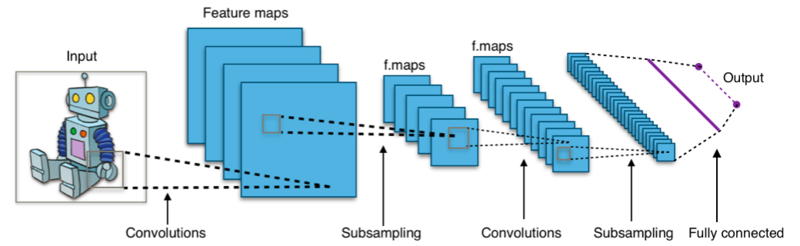
\includegraphics[width=0.8\columnwidth]{docs/Typical_cnn.png} 
\caption{Typical CNN}
\label{fig_typicalCNN}
\end{figure}

The three operations mentioned before (convolution, activation function and pooling) are the set of mathematical ingredients that are used in any CNN to process and classify images.


\subsection{Convolution}
given an image \( I \epsilon R^{n \cdot m}  \) and a filter  \( K \epsilon R^{k \cdot k}  \) the resulting pixel of this operation \( I_{x,y} * K \) (which is a 2D convolution) is the result of the following equation:
\begin{equation} 
\label{conv1}
Ic_{(x,y)} = I_{x,y} * K = \sum_{u=-k/2}^{k/2}\sum_{v=-k/2}^{k/2}K_{u,v} \cdot I_{x-u,y-v}
 \end{equation}
The equation (1) requires to flip the filter K and to center it on the target pixel \( I_{x,y} \), if you consider the filter as a set of weights then the resulting pixel \( Ic_{(x,y)} \) is just a weighted sum of the input pixel \( I_{x,y} \) and the surrounding ones.\\
Due to the fact that in a CNN the filter can be considered already inverted and not all input pixels are convoluted but only those in the central portion of the image where the filter doesn't go out of border: \[x \in [k/2,m-k/2], y \in [k/2, n-k/2] \] the operation can be simplified as a standard dot product:
\begin{equation}
\label{conv2}
Ic_{(x,y)} = \sum_{u=0}^{k}\sum_{v=0}^{k}K_{u,v} \cdot I_{x+u,y+v}
 \end{equation}
Just to be clear, the following example makes use of the equation (1) where for simplicity the filter K is the identity filter (in this case the inverted version K' is the same K):
\[
I
\left(
\begin{array}{ccccccc}
  1&   2&  3&   4&   5&   6  \\
  7&   8&  9&  10&  11& 12         \\
  13&   14& 15& 16& 17& 18  \\
  19&   20& 21& 22& 23& 24 \\
  25&   26& 27& 28& 29& 30  \\
  31&   32& 33& 34& 35& 36 \\
\end{array}
\right)
*
K
\left(
\begin{array}{ccc}
  0&   0&  0 \\
  0&   1&  0 \\
  0&   0& 0 
\end{array}
\right)
=
\left(
\begin{array}{ccccccc}
  1&   2&  3&   4&   5&   6  \\
  7&   8&  9&  10&  11& 12         \\
  13&   14& 15& 16& 17& 18  \\
  19&   20& 21& 22& 23& 24 \\
  25&   26& 27& 28& 29& 30  \\
  31&   32& 33& 34& 35& 36 \\
\end{array}
\right)
\]

The following example makes use of the equation (2) with the same I, K:
\[
I
\left(
\begin{array}{ccccccc}
  1&   2&  3&   4&   5&   6  \\
  7&   8&  9&  10&  11& 12         \\
  13&   14& 15& 16& 17& 18  \\
  19&   20& 21& 22& 23& 24 \\
  25&   26& 27& 28& 29& 30  \\
  31&   32& 33& 34& 35& 36 \\
\end{array}
\right)
*
K
\left(
\begin{array}{ccc}
  0&   0&  0 \\
  0&   1&  0 \\
  0&   0& 0 
\end{array}
\right)
=
\left(
\begin{array}{ccccc}
  8&  9&  10&  11 \\
  14& 15& 16& 17  \\
  20& 21& 22& 23 \\
  26& 27& 28& 29 \\
\end{array}
\right)
\]

This is the formula used to compute the output matrix's size Os starting from input matrix's size Is and filter's size Ks:
\begin{equation} 
\label{outsize}
Os = Is - Ks +1
 \end{equation}

\subsection{Activation Function}
The activation function, sometimes also called transfer function, defines how the weighted sum of the input (so the result of a convolution) is transformed into an output value.\\
There are different types of activation functions and usually many of them are nonlinear functions,  and the choice of which activation function to use can really affects the performances and the capabilities of a neural network.\\
Typically every pixel after being convoluted is also activated, this operation is performed by the convolution layers.\\
Without going into many details, the LeNet-1 makes use of the Sigmoid function which is the following nonlinear function:
\begin{equation} 
\label{outsize}
S(x) = \frac{1}{1+e^{-x}}
 \end{equation}
 
\begin{figure}[h]
\centering
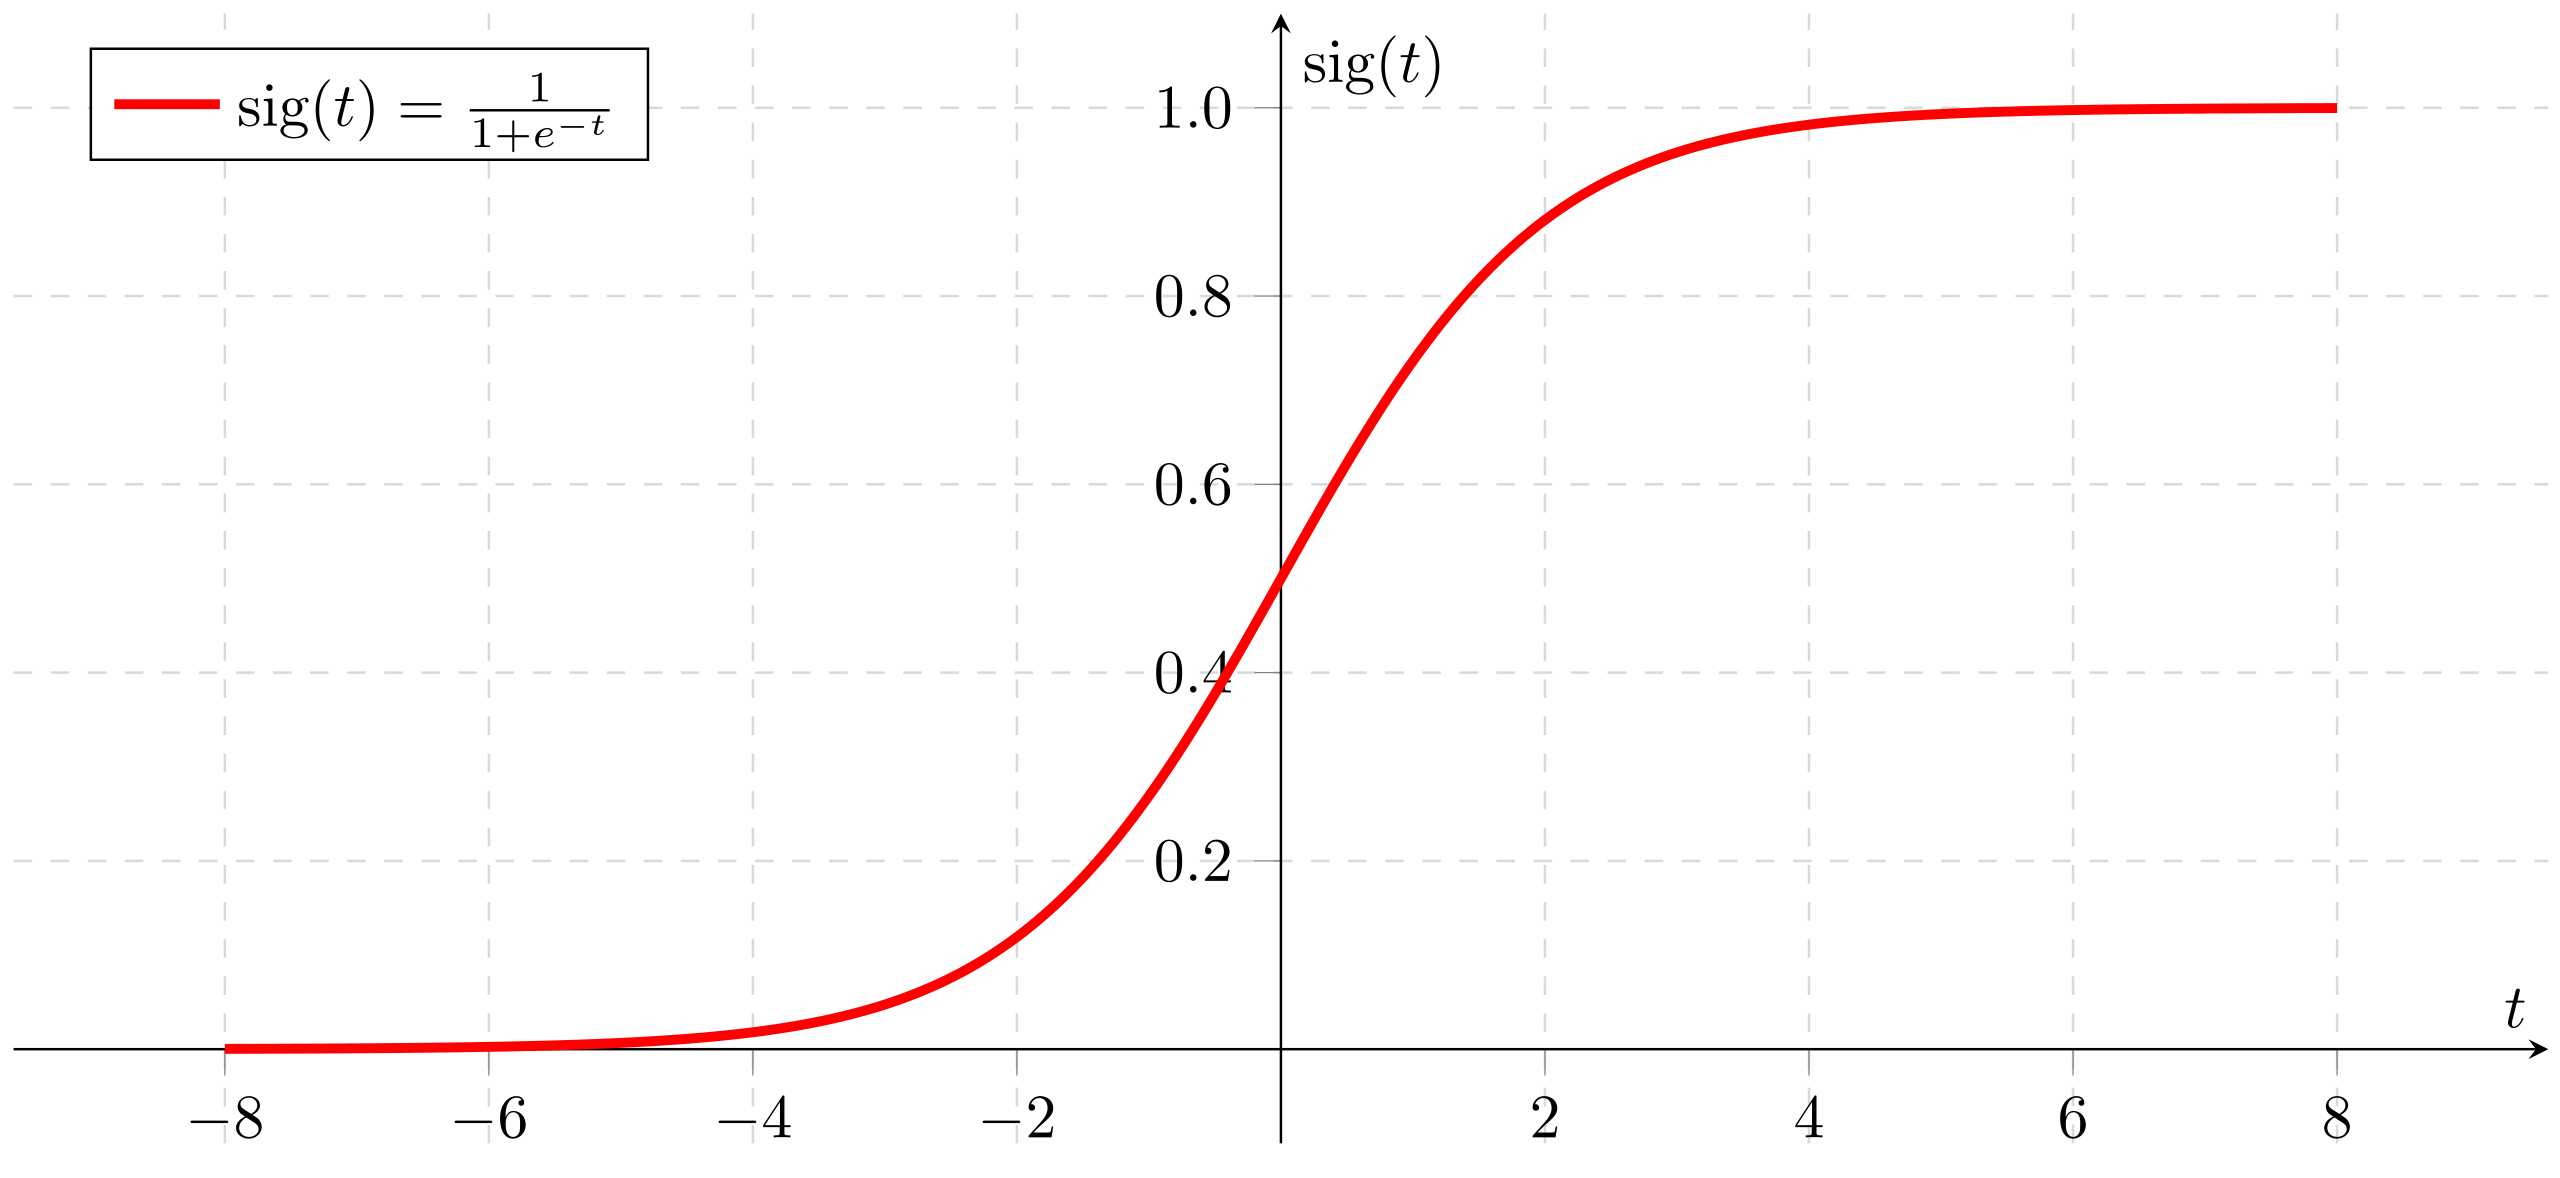
\includegraphics[width=0.8\columnwidth]{docs/sigmoid.png} 
\caption{Sigmoid activation function}
\label{fig_sigmoid}
\end{figure}
 

\subsection{Pooling Function}
Another widely used operation in a CNN is the Pooling function also called Subsampling function.\\
Pooling is a sample-based discretisation process with the aim of down-sample an input representation (image, hidden-layer, generic matrix, etc) and so reducing it's dimensionality.\\
The basic procedure of pooling is very similar to the convolution operation. You select a filter, you slide it over the input representation and you obtain a new output representation.\\
In this case the most commonly used filter size is 2x2 and the filter is slid over the input pixels with a stride of 2.\\\\\\\\
There are several approaches to pooling, the most commonly used are the following two:

\begin{itemize}  
\item Max Pooling: \\
the filter simply selects the maximum pixel value in the 2x2 region\\
example:\\
\[
\left(
\begin{array}{ccccc}
  8&  9&  10&  11 \\
  14& 15& 16& 17  \\
  20& 21& 22& 23 \\
  26& 27& 28& 29 \\
\end{array}
\right)
\mapsto
\left(
\begin{array}{cc}
  15&  17  \\
  27& 29
\end{array}
\right)
\]
\item Average Pooling: \\
in this case the pooling works by calculating the average value of the pixels in the 2x2 region\\
example:\\
\[
\left(
\begin{array}{ccccc}
  8&  9&  10&  11 \\
  14& 15& 16& 17  \\
  20& 21& 22& 23 \\
  26& 27& 28& 29 \\
\end{array}
\right)
\mapsto
\left(
\begin{array}{cc}
  11.5&  13.5  \\
  23.5& 25.5
\end{array}
\right)
\]
\end{itemize}

Right now, many implementations use max pooling because it is less expensive from a computationally point of view and it can helps in speeding up the CNN.


%%%CAP 3 PROJECT DESCRIPTION %%%%%
\section{LeNet-1 Architecture}
Now that all the mathematical basics were briefly introduced the discussion can finally introduce the forward propagation algorithm of the LeNet-1 CNN.\\
\begin{figure}[!h]
\centering
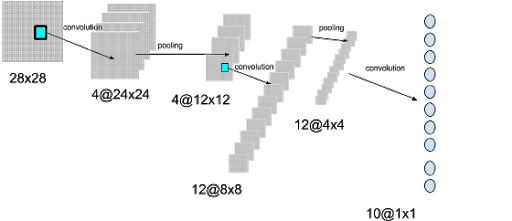
\includegraphics[width=0.8\columnwidth]{docs/LeNet1.png} 
\caption{Anatomy of the LeNet-1}
\label{fig_lenet}
\end{figure}

From Figure 3 it is possible to observe that, starting from the input layer, the overall architecture is composed of 3 convolutional layers and 2 pooling layers for a total amount of 4 hidden layers and a final output layer.
\begin{enumerate}
\item Input Layer: \\
consists of a 28x28 image that represents the first 784 input neurons.
\item First Hidden layer: \\
First convolutional layer composed of four 24x24 feature maps that forms a group of 2304 neurons.
\item Second Hidden layer:\\
First average pooling layer composed of four 12x12 feature maps that forms a group of 576 neurons.
\item Third Hidden layer:\\
Second convolutional layer composed of twelve 8x8 feature maps that forms a group of 768 neurons.
\item Fourth Hidden layer:\\
Second and last average pooling layer composed of twelve 4x4 feature maps that forms a group of 192 neurons.
\item Output layer:\\
Contains the result of the classification of the input image. This CNN as said in the Introduction is meant to be used to classify digits between 0-9, so the output layer contains the classification on a 10x1 array.
\end{enumerate}


\subsection{Description of the first hidden layer}
Starting from the input image, four filters K1, K2, K3, K4 of size 5x5 (25 weights each) are convoluted to generate the four feature maps.\\
The size of each feature map is 24x24 and can be easily computed with the equation (3) where Is=28 and Ks=5.\\
The visual representation of the first convolutional layer is showed in Figure 4.\\
The values of the first layer are instead given by the following equation:
\begin{equation} 
\label{convLayer}
F^{s}_{x,y} = \sigma (bias + \sum_{u=0}^{4}\sum_{v=0}^{4}K^{s}_{u,v} \cdot I_{x+u,y+v})
 \end{equation}

Where \( F^{s}_{x,y} \) is the (x,y) neuron of the s-th feature, \( \sigma \) is the Sigmoid activation function in the equation (4) that transform the result of convolution (equation (2)) plus a bias term.\\
The remaining parts of the equation are the term \( K^{s}_{u,v} \) that is the (u,v) weight of the s-th filter, and finally \( I_{x+u,y+v} \) is the (x+u,y+v) pixel of the input image.\\\\\\\\
\begin{figure}[!h]
\centering
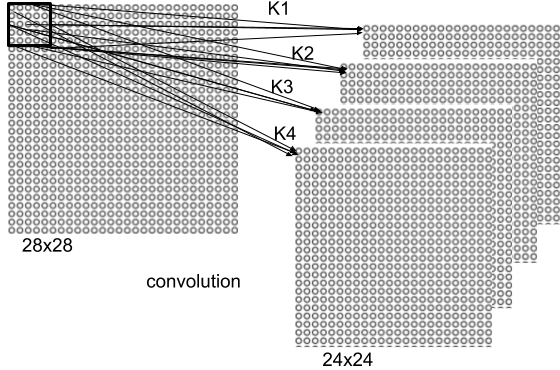
\includegraphics[scale=0.3]{docs/c1.png} 
\caption{First convolutional layer, first hidden layer}
\label{fig_c1}
\end{figure}

\subsection{All layers}
Stated that LeNet-1 has an overall of three convolutional layers and two pooling layers, the network can be described by the following flow:
\[ INPUT \mapsto C1 \mapsto S1 \mapsto C2 \mapsto S2 \mapsto C3 \mapsto OUTPUT \]
Once the input has been convoluted into four feature maps, each feature map is pooled into 4 corresponding feature maps of 12x12 each.\\
In the next layer, the third hidden layer, the convolution is done again by the same equation (5) but this time there are only 3 filters 5x5.
Since the three filters are convoluted on each of the four feature maps, this multiplies the amount of feature maps of the next layer to 12.
Now the new layer is pooled again and by doing that the last hidden layer is created and the size is reduced from 768 to 192 neurons that correspond to the last 12 4x4 features in the hidden layers.\\
To fully connect the last hidden layer to the 10 output neurons one last convolution is used, in particular each \( Out_{i} \) can be computed using this formula:
\begin{equation} 
\label{fullyConn}
Out_{i} = \sigma (bias + \sum_{j=0}^{11}K_{i}  * F_{j})
 \end{equation}
 
 where \( \sigma \) is the usual Sigmoid, \( K_{i} \) is the i-th filter over the total 10 of the last convolutional layer and  \( F_{j} \) is the j-th feature map of the last hidden layer.\\
The following image can help to understand how the last hidden layer is fully connected to the ouput:

\begin{figure}[!h]
\centering
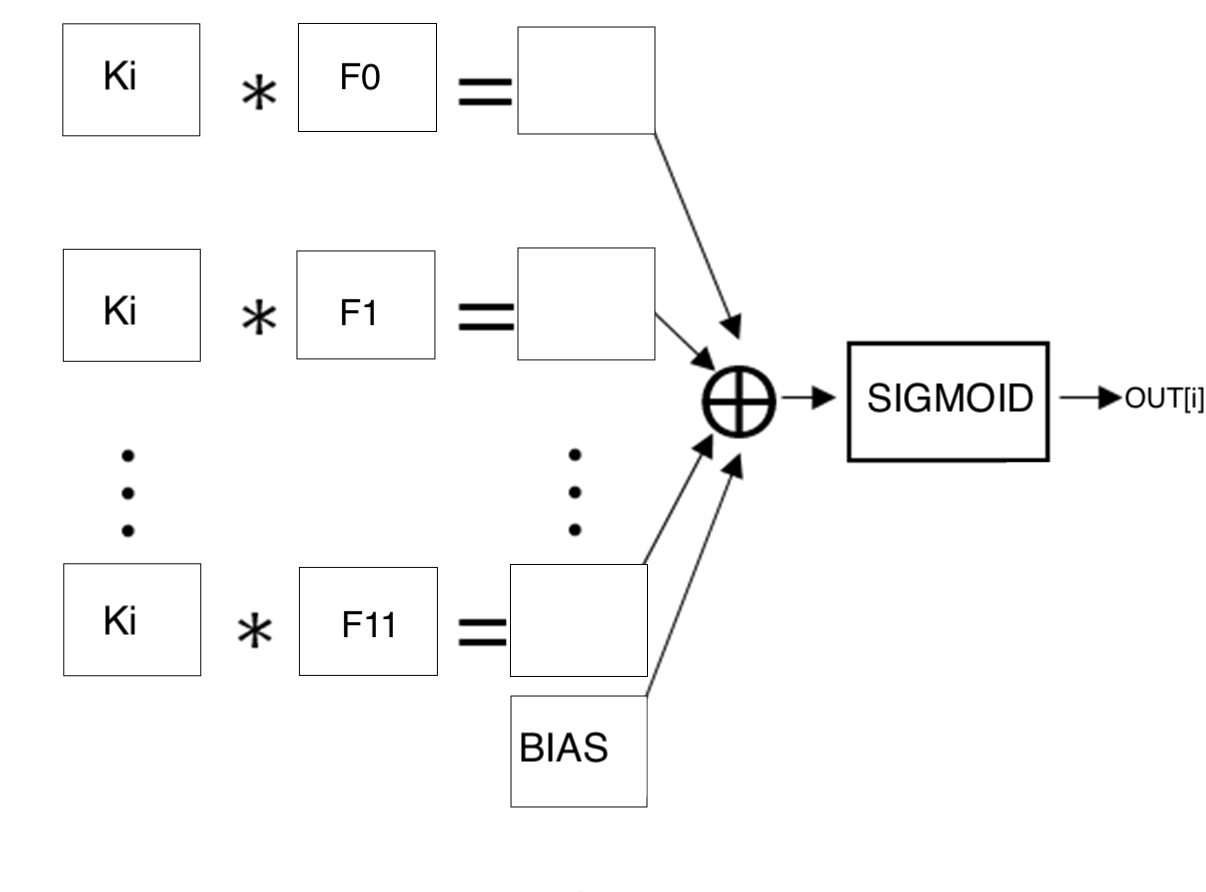
\includegraphics[scale=0.7]{docs/c3.png} 
\caption{Third convolutional layer, Fully connected to output layer}
\label{fig_c3}
\end{figure}

\subsection{Other comments about LeNet}
Even if the architecture of the LeNet-1 CNN is a very simple example without too many hidden layers and features it is important to underline that every forward propagation (every image classification) requires a big set of operations that are sequences of multiplications, additions, divisions and exponentials.
All the mentioned operations repeated for every neuron inside the network will require hundreds of thousands of floating point operation and this render the problem heavy from a computational point of view!

\section{Implementation}
The board used for implementing and testing the forward propagation algorithm is the NVIDIA Jetson Nano.\\
First of all the forward propagation was implemented on the CPU (host) to have a reference benchmark of the algorithm executed serially, then the code was ported on the GPU (device).\\
Concerning the device implementation there are three solution proposed:
\begin{enumerate}
\item heavy usage of global memory, all the weights are saved in global memory and all feature maps are processed in global memory.
\item filters are moved in constant memory space, in such a way to reduce the global memory usage.
\item soft usage of global memory, all computations in shared memory, filters in constant memory.
\end{enumerate}

\subsection{CPU implementation \& serial benchmarks}
The host code is very simple, it serially executes this series of transformation already discussed in the previous sections:
\[ Image28x28 \mapsto C1_{4x24x24} \mapsto S1_{4x12x12} \mapsto C2_{12x8x8} \mapsto S2_{12x4x4} \mapsto C3_{10x1x1} \mapsto OUTPUT \]
The following graph is showing the execution times for 10 consecutive forward propagations randomly selected among 50000 recorded executions of the algorithm with random images and random weights:

\begin{figure}[!h]
\centering
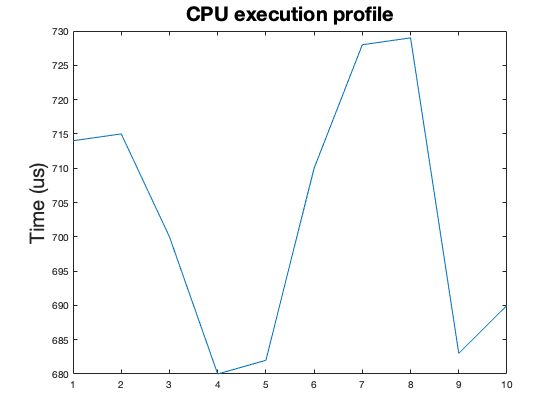
\includegraphics[scale=0.5]{docs/hostexec.png} 
\caption{CPU performance profile}
\label{fig_hp}
\end{figure}

\subsection{GPU implementations}
Considering that the propagation through the layers is sequential it is still possible to accelerate the overall performances of the network by speeding-up the internal operations of each layer.\\
Once the features of the layer \( i \) are ready, all the features of the layer \( i+1 \) can be processed in parallel because each neuron can be computed independently from all others in the same layer.\\
As introduced before, the implementation starts from a very naïve version that processes data using heavily the global memory, the goal was to move as much as possible the data in shared memory in such a way to reduce as much as possible the amount of global memory transactions.\\
The algorithm is executed by a single block of 28x28 threads and it is the same in all the 3 versions, the only differences are how the data are arranged in the memories.

\subsection{Naïve version benchmarks}
All filters are saved in global memory, all features are saved in global memory.
Data arranged like this will produce a lot of transactions because each feature, once computed, needs to be stored in global memory in such a way that can be used to feed the next layer when the propagation moves forward, and also the efficiency of the transaction will not be optimal because of the strided accesses by convolution and pooling operations.\\
The following metrics were collected by using the profiler:

\begin{table}[!h]
\centering
\begin{tabular}{|l|l|l|l|l|}
\hline
\textbf{Kernel Name} & \textbf{load efficiency} & \textbf{store efficiency} & \textbf{load transactions} & \textbf{store transactions} \\ \hline
deviceForwardV1           & 49.17\%           & 76.15\%           & 124610           & 632       \\ \hline
\end{tabular}
\vspace*{3mm}
\caption{Naïve version Global memory profile}
\label{table:t1}
\end{table}

In the following table are shown the performances of the kernel collected again with the profiler.\\
Note that not only the pure kernel execution time is considered but also the CUDA APIs calls are considered in the final execution time.
The API calls are the following ones: \( memcpy HostToDevice \) ,  \( memcpyDeviceToHost \) and the \( cudaDeviceSynchronize \).\\
The total execution time is then the time the processor needs to wait in order to be able to use the GPU results.

\begin{table}[!h]
\centering
\begin{tabular}{|r|r|r|r|}
\hline
\textbf{Kernel Name} & \textbf{Avg. kernel exec time} & \textbf{Avg. APIs overhead} & \textbf{Avg. total exec time} \\ \hline
deviceForwardV1           & 370us          & 540us   & 900us\\ \hline
\end{tabular}
\vspace*{3mm}
\caption{Naïve version performances}
\label{table:t2}
\end{table}

Is possible to see that even if the algorithm is executed faster on the GPU (370us against 700us in Figure 6) the overall execution time is expected to be on average higher than the CPU one.\\
The following picture shows a comparison between CPU and Naïve version performances (again using 10 random execution times among a collection of 50000):

\begin{figure}[!h]
\centering
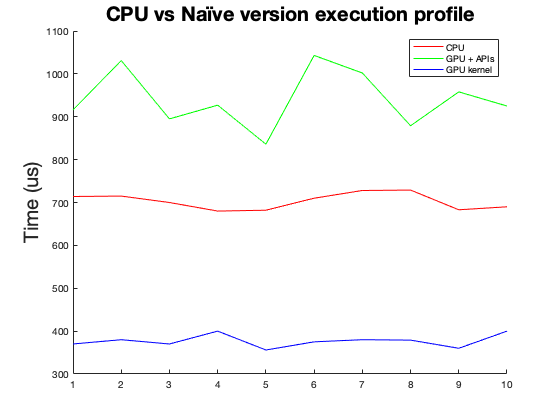
\includegraphics[scale=0.5]{docs/cpuVSnaive.png} 
\caption{CPU vs GPU performances, version 1}
\label{fig_gpu1}
\end{figure}

\subsection{Constant memory version benchmarks}
Considering that once a network is trained all the filters are maintained constant, is possible to take advantage of the Constant Memory.\\
The only data that needs to be moved in and out form the global memory are then only the features, the profiler already shows a significant reduction of the global transactions:

\begin{table}[!h]
\centering
\begin{tabular}{|l|l|l|l|l|}
\hline
\textbf{Kernel Name} & \textbf{load efficiency} & \textbf{store efficiency} & \textbf{load transactions} & \textbf{store transactions} \\ \hline
deviceForwardV2           & 59.45\%           & 76.15\%           & 64610           & 632       \\ \hline
\end{tabular}
\vspace*{3mm}
\caption{Constant memory version Global memory profile}
\label{table:t3}
\end{table}

The performances are now expected to be better, in fact the profiler shows the following results:

\begin{table}[!h]
\centering
\begin{tabular}{|r|r|r|r|}
\hline
\textbf{Kernel Name} & \textbf{Avg. kernel exec time} & \textbf{Avg. APIs overhead} & \textbf{Avg. total exec time} \\ \hline
deviceForwardV2           & 283us          & 370us   & 650us\\ \hline
\end{tabular}
\vspace*{3mm}
\caption{Constant memory  performances}
\label{table:t4}
\end{table}

The new version is roughly 30\% faster than the Naïve one but even if overall execution time is not much better that the CPU's.\\ 
The results confirms that the approach of reducing the global memory usage is the right one!\\

\begin{figure}[!h]
\centering
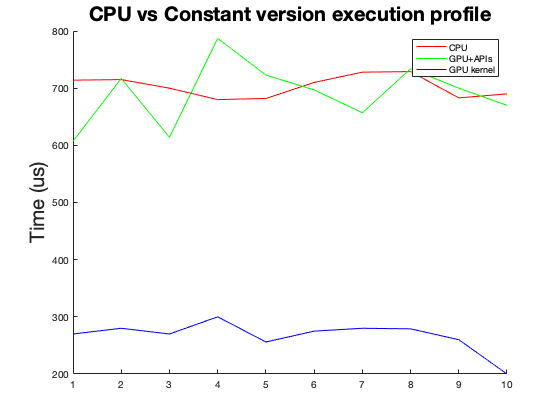
\includegraphics[scale=0.5]{docs/cpuVSconstant.png} 
\caption{CPU vs GPU performances, version 2}
\label{fig_gpu2}
\end{figure}

\subsection{Shared \& Constant memory version benchmarks}
This is the final implementation of the algorithm, in the previous one the filters have been removed from global memory, now considering that:

\begin{enumerate}
\item there is only a single block running on the GPU, this means that all threads can easily work together using the same data in shared memory.
\item all the features together occupy a total amount of: \( (4x24x24 + 4x12x12 + 12x8x8 + 12x4x4) \cdot 4  \approx 16 Kbytes\), our device has 49 Kbytes of shared memory per block so the entire features can be stored in shared memory.
\item the kernel just needs the input image and needs to provide to the CPU just the output layer.
\end{enumerate}

all the computations can be done using just the shared + constant memory, the overall usage of global memory is negligible because only transactions issued are for loading the input layer in shared memory and storing the output layer in global memory:

\begin{table}[!h]
\centering
\begin{tabular}{|l|l|l|l|l|}
\hline
\textbf{Kernel Name} & \textbf{load efficiency} & \textbf{store efficiency} & \textbf{load transactions} & \textbf{store transactions} \\ \hline
deviceForwardV3           & 100.00\%           & 62.50\%           & 394           & 2       \\ \hline
\end{tabular}
\vspace*{3mm}
\caption{Constant + Shared version, Global memory profile}
\label{table:t5}
\end{table}

Also the shared memory usage showed good results in terms of bank conflicts, the following metrics and events have been profiled:

\begin{table}[!h]
\centering
\begin{tabular}{|l|l|l|l|l|}
\hline
\textbf{ld. transactions/request} & \textbf{st. transactions/request} & \textbf{ld. bank conflicts} & \textbf{st. bank conflicts}  \\ \hline
1.026161           & 1.023599           & 0           & 8          \\ \hline
\end{tabular}
\vspace*{3mm}
\caption{Constant + Shared version, Shared memory profile}
\label{table:t6}
\end{table}

The performances showed overall better results: 

\begin{table}[!h]
\centering
\begin{tabular}{|r|r|r|r|}
\hline
\textbf{Kernel Name} & \textbf{Avg. kernel exec time} & \textbf{Avg. APIs overhead} & \textbf{Avg. total exec time} \\ \hline
deviceForwardV3           & 172us          & 230us   & 400us\\ \hline
\end{tabular}
\vspace*{3mm}
\caption{Constant memory  performances}
\label{table:t7}
\end{table}

The new version is expected to roughly 2x faster that the CPU one.

\begin{figure}[!h]
\centering
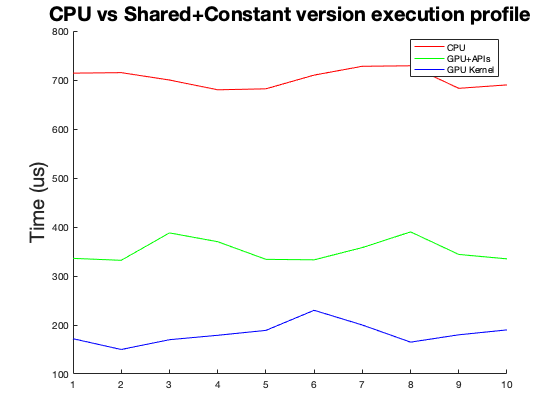
\includegraphics[scale=0.6]{docs/cpuVSshared.png} 
\caption{CPU vs GPU performances, version 3}
\label{fig_gpu3}
\end{figure}

%In this final image are showed together the performances of the 3 versions to have a better idea of the achieved results:

%\begin{figure}[!h]
%\centering
%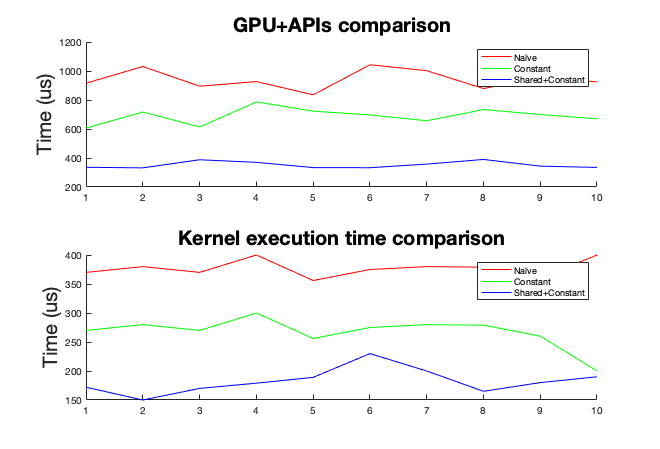
\includegraphics[scale=0.5]{docs/finalCmp.png} 
%\caption{Comparison between GPU versions}
%\label{fig_gpu4}
%\end{figure}

\section{Final comments}
The different implementations can show how is possible to speed up an algorithm by just take advantage of the different memory hierarchies in the device.\\
The issue behind the implementations presented before is connected to the device occupancy, which is a very important metric that indicates how many warps are active out of the total amount supported by the multirocessor(s) on the GPU.
Even if the final version is optimised from a memory point of view, the overall occupancy is low, around 40\%, because the more the propagation moves across the layers the less threads will work.\\
So next steps would be trying to design a solution that increases as much as possible the device occupancy by using for example multiple blocks instead of 1.

\section{References}

\begin{enumerate}
\item Anatomy of the LeNet-1 Neural Network: https://acodez.in/anatomy-of-the-lenet-1-neural-network/
\item Review LeNet-1: https://sh-tsang.medium.com/paper-brief-review-of-lenet-1-lenet-4-lenet-5-boosted-lenet-4-image-classification-1f5f809dbf17
\item Anatomy of the LeNet-1 CNN: https://www.skyradar.com/blog/anatomy-of-the-lenet-1-convolutional-network-and-how-it-can-be-used-in-order-to-classify-radar-data
\item Professional CUDA C Programming
\end{enumerate}




\end{document}